\documentclass[a4paper,12pt,oneside,uplatex]{jsarticle}
\usepackage[utf8]{inputenc}
\usepackage[english]{babel}
\usepackage{csquotes}
\usepackage{biblatex}
\addbibresource{./reference.bib}
\usepackage[papersize={210truemm, 297truemm}]{geometry}
\geometry{top=40truemm,bottom=35truemm,left=25truemm,right=25truemm}
%
\usepackage[utf8]{inputenc}
\usepackage{booktabs}
\usepackage{url}
\usepackage{nidanfloat}
\usepackage{afterpage}
\usepackage{setspace}
\usepackage{multirow}
\usepackage{here}
\usepackage{geometry}

\usepackage{amsmath,amssymb}
\usepackage{bm}
%\usepackage{graphicx}
\usepackage[dvipdfmx]{graphicx}
\usepackage{verbatim}
\usepackage{wrapfig}
\usepackage{ascmac}

\usepackage{algorithm}
\usepackage{algorithmic}

\usepackage{bxwareki}
\usepackage{okumacro}

%
\setcounter{tocdepth}{3}
%
%余白設定
\setlength{\textwidth}{\fullwidth}
\setlength{\textheight}{35\baselineskip}
\addtolength{\textheight}{\topskip}
\setlength{\voffset}{-0.55in}
\setlength{\abovedisplayskip}{2.5pt} % 上部のマージン
\setlength{\belowdisplayskip}{2pt} % 下部のマージン
%
\newcommand{\etal}{\textit{et al}.,}
\newcommand{\ie}{\textit{i}.\textit{e}.,}
\newcommand{\eg}{\textit{e}.\textit{g}.,}
\newcommand{\reffig}[1]{Fig.\ref{#1}}
\newcommand{\reftab}[1]{Table.\ref{#1}}
\newcommand{\refequ}[1]{Formula.\ref{#1}}
\newcommand{\refsec}[1]{Section.\ref{#1}}

%%%%%%%%%%%%%%%%%%%%%%%%%%%%%%%%%%%%%%%%%%%%%%%%%%%%%%
\title{The New Fake News Classification with Comment Generation by Seq-GAN}
\author{Yuta Yanagi}
\date{\today}
\begin{document}
\include{front}
%
%\maketitle
%
%\frontmatter
%表紙
\begin{titlepage}
  \vspace*{7mm}
  \begin{center}
    \Large{Masters Thesis Proposal}\\

    \vspace{40truemm}

    \LARGE{\textbf{The New Fake News Classification with Comment Generation by Seq-GAN}}\\

    \vspace{30truemm}

    \Large{Yuta Yanagi}\\
    \Large{Department of Informatics, The University of Electro-Communications}\\

    \vspace{15truemm}

    \begin{table*}[h]
        \centering
        \hspace*{4em}
        \begin{tabular}{rcl}
            \large{Main Advisor}&\large{:}&\large{Yasuyuki Tahara} \vspace{5truemm} \\
            \large{Advisor}&\large{:}&\large{Akihito Ohsuga} \vspace{5truemm} \\
            \large{Advisor}&\large{:}&\large{Yuichi Sei} \vspace{5truemm} \\
        \end{tabular}
    \end{table*}
  \end{center}
\end{titlepage}
%
%アブスト

\section{Abstract}
%
%本文
\section{Introduction}
In this era, social media is one of important parts of our lives.
Social media makes more easy to get news and share with friends online.
However, at the same moment, 
there are also information includes less credibility.
Some of them have obvious misinformation that are made by malicious purpose,
we call them ``fake news''.

Fake news try to make wrong rumors on social media by spreading on social media.
Last year, a picture was spread on Russian social media which shows someone with an Estonian flag on their sleeve beating the protester.
After this, Estonian volunteers identified this picture as a fake news\cite{vaikmaa_2019}.
In addition, In the U.S., fake news created some mayhem not only online, but also offline(real incidents)
e.g. in Washington, fake news about the Pizzagate conspiracy is reported to have motivated the shooting\cite{agencies_2016}.
Spreading fake news also shakes premise of democracy due to people cannot get accurate information.
Therefore, there are some researches which try to spot fake news by machine learning.

The challenging point of this is there are news article which try to deceive readers
and this makes harder to classify by simple rule-based method.
To get more information to detection,
there are some works which aggregate social context i.e. Retweet, Like, and comments
report better results than only considering news text\cite{Guo:2018:RDH:3269206.3271709}.
However, social contexts are not able to get before spreading.
Hence, there is also a work which generate words of comments from news by CVAE to detect fake news when they are just posted\cite{ijcai2018-533}.
Their work tries to generate comments, but generated ones are only have words which have high probability of appearing.

In this work, We will propose a model which evaluate news credibility by news text and generated comments by Seq-GAN\cite{Yu:2017:SSG:3298483.3298649}.
This model train not only news features but also generating comments.
In training sequence includes real posted comments but test sequence doesn't use them in order to simulate operation in real-social media.
The skill of generating comments help classification in test sequence.

We plan to measure performance of our proposed method by some experiments with real-posted dataset and some state-of-the-art fake news detection algorithms.

\section{Related Works}
\section{Thesis}
The main objective of this research is developing new fake news classification 
with comment generation and investigate how proposed method is better in operation on social media.
To suppress spread of fake news, we have to spot it early enough.
Specifically, it is required classifying before spread of fake news if classifier operate in social media.

In classification of fake news, social contexts give strong information.
Among social contexts, comments gives more information as natural language than retweets and likes.
However, it is impossible to get social contexts from news which is just posted on social media.
Therefore, we train model not only classifier but also comment generator for fake news detection.
This use Seq-GAN \cite{Yu:2017:SSG:3298483.3298649} as comment generation with real comments which are posted in Twitter.
\section{Methodology}
Our proposed model structure is very similar to Seq-GAN\cite{Yu:2017:SSG:3298483.3298649} and 
it has classifier and comment generator.
\reffig{fig:structure} shows structure of our model.
On the one hand, generator create comments from post.
On the other hand, classifier evaluates two values to binary classifications with real or generated comments from generator: 
post's credibility and reality of comments.

\begin{figure}[ht]
    \centering
    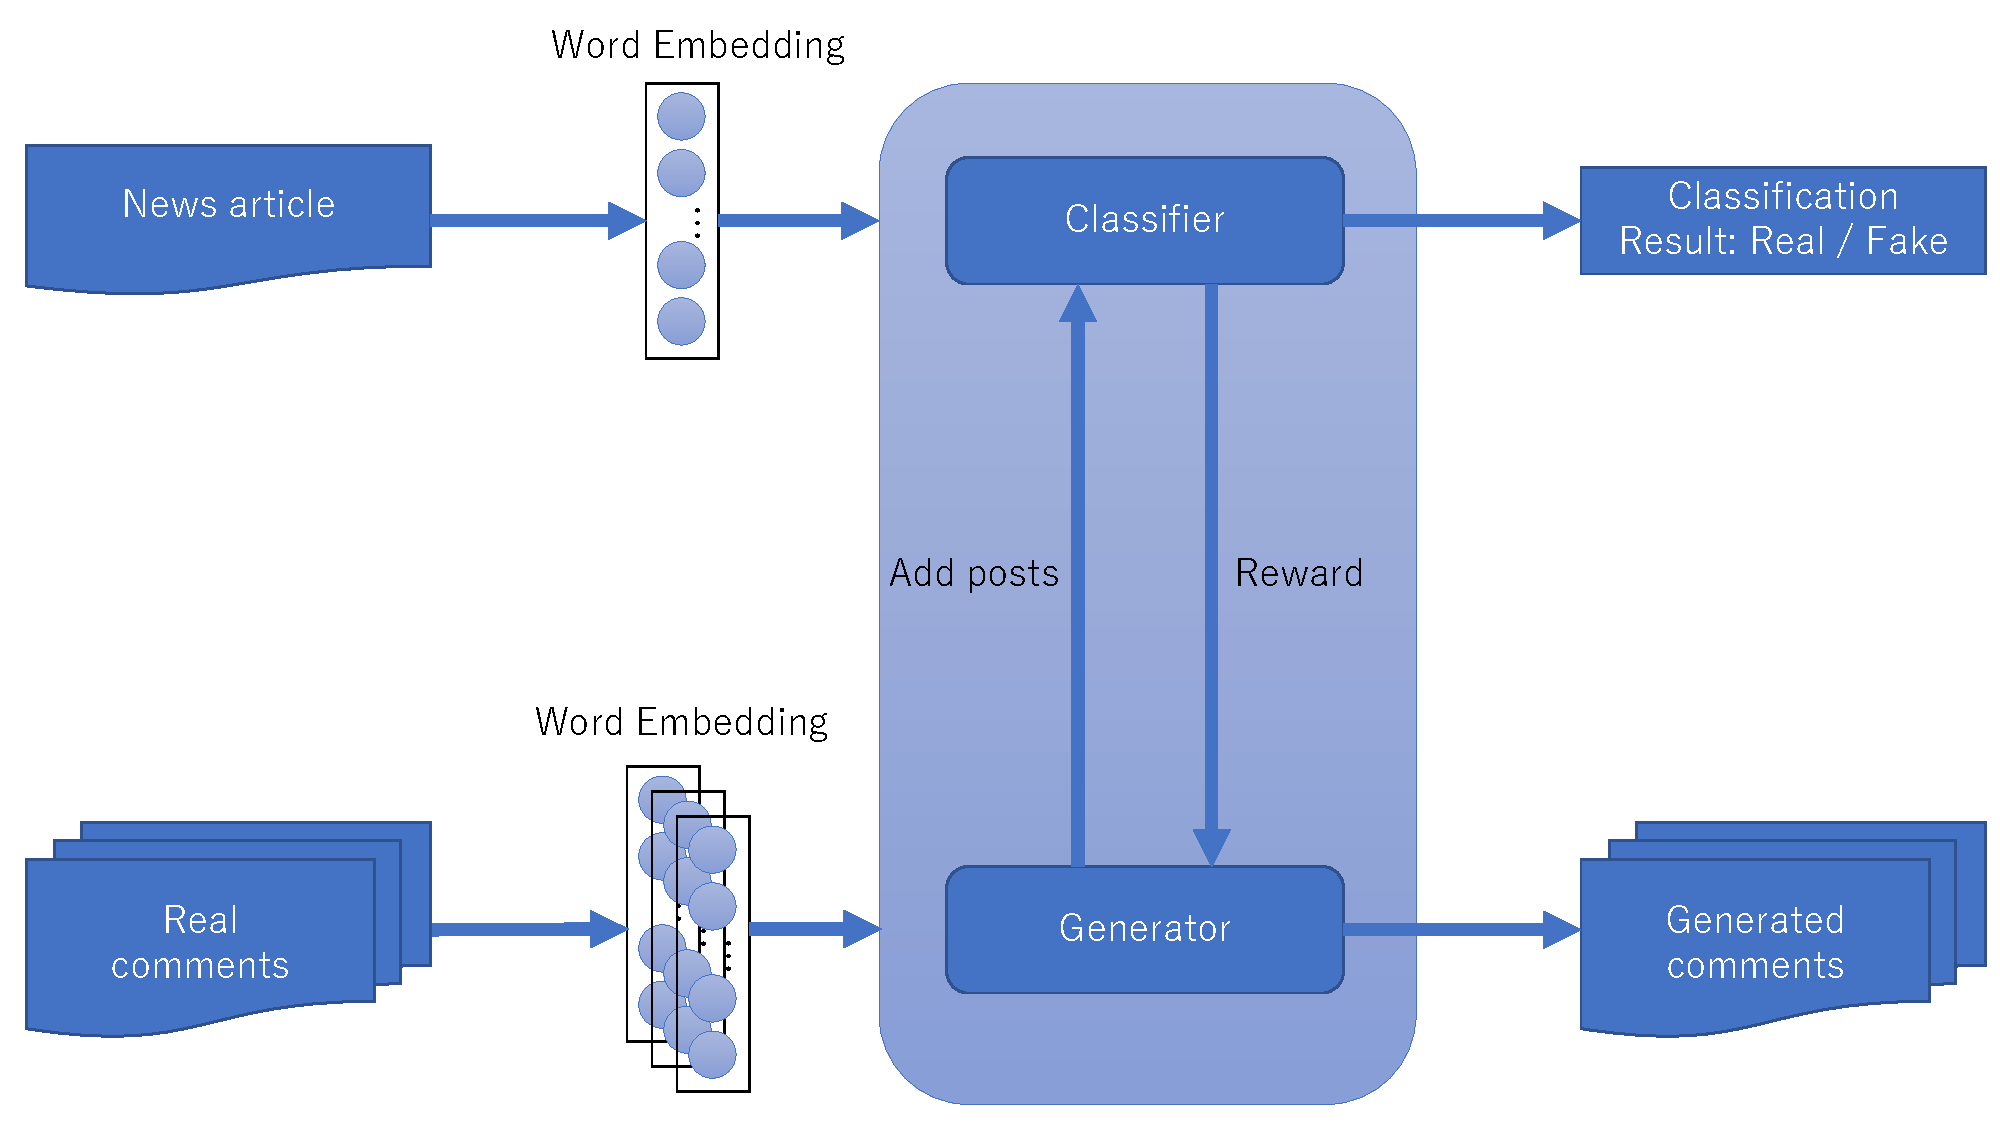
\includegraphics[width=0.85\textwidth]{images/research_proposal_structure.pdf}
    \caption{The structure of our planning proposed model.}
    \label{fig:structure}
\end{figure}

Generator is trained by post feature which is leaked from classifier and
classifier is trained by label of posts(true, fake) and comments(real, generated).
In the test term, classifier only use posts with generated comments in order to
simulate operation on social media.
\section{Preliminary Results and Discussion}
\subsection{Dataset}
In order to input our proposed model, we obtained FakeNewsNet\cite{shu2017exploiting,Shu:2017:FND:3137597.3137600,shu2018fakenewsnet} dataset.
This includes tweets which has URL of news.
Every news and tweets are labeled true/fake by fact-check result on PolitiFact or GossipCop.
We use tweet text as comments and the other information(user, retweet, like, etc.) are not used.
\reftab{table:fakenewsnet} is statistics of dataset.

\begin{table}[htp]
    \centering
    \caption{Statistics of FakeNewsNet by fact-checking platforms}
    \label{table:fakenewsnet}
    \begin{tabular}{lcccc}
        \hline 
        & \multicolumn{2}{c}{True} & \multicolumn{2}{c}{Fake} \\
        Platform & News & Comments & News & Comments \\
        \hline \hline 
        PolitiFact & 624 & 370669 & 432 & 195901 \\
        GossipCop & 16817 & 843933 & 5323 & 539491 \\
        \hline 
        Overall & 17441 & 1214602 & 5755 & 735392 \\
        \hline 
    \end{tabular}
\end{table}

\subsection{Plan of experiments}
We will make answer of following evaluation questions:
\begin{description}
    \item[EQ1] Can our proposed model detect fake news more accurate than any other state-of-the-art fake news detection algorithms?
    \item[EQ2] Is generating comments important in fake news detection by Seq-GAN?
    \item[EQ3] Are generated comments similar to real comments?
\end{description}

We are planning to answer them by comparing our model with any other state-of-the-art fake news detection algorithms,
ablation experiments, and subjective evaluation by human beings.

\subsection{Plan of discussion}
\subsubsection{EQ1: comparing}
We will get results of not only our proposed model but also other algorithms which are proposed by related works.
All of them use both of news text and comments for equal comparing.
\subsubsection{EQ2: ablation experiments}
We also compare by ablation experiments.
It does our proposed model with ones which don't use generated comments in order to
testify to importance of generating comments by Seq-GAN.
If proposed model is better than ablated one, generating comments is important part to find fake news.
\subsubsection{EQ3: subjective evaluation}
When training is over, generated comments will be so similar to real comments.
We can measure how far from real comments to generated comments are by subjective evaluation.
\section{Implications of Research}
This research will show how generating comment is important to identify fake news on social media.
Fake news constitutes a grave menace to the safety of our world, we fear.
Therefore, it is important to detect news credibility before spreading on social media.
We aim to detect fake news more precisely by generating comments from articles that are only available after they have spread.

In computer science, computer security is the protection of computer systems.
Likewise, countering to fake news prevent people from exposing to malicious information on social media.
This is similar to computer security for the purpose of protecting the safety of society.

%謝辞
%\input{./sections/thanks}

%参考文献
\newpage
\addcontentsline{toc}{section}{reference}
\printbibliography

%付録
%\input{./sections/appendix}
%
%
\end{document}